\documentclass[12pt,a4paper]{article}

\usepackage{array}
\usepackage{amssymb}
\usepackage{amsfonts}
\usepackage{graphicx}
\usepackage[sans]{dsfont}
\usepackage{bbm}
\usepackage{amsmath,bm}
\usepackage{url}
\usepackage{hyperref}
\usepackage{eurosym}
\usepackage{mathtools}

\usepackage[top=2cm, bottom=2cm, left=2cm, right=2cm]{geometry}
\usepackage[dvipsnames]{xcolor}

\title{Triangle problem}

\begin{document}
\maketitle

\section{The problem}

\begin{figure}[th]
  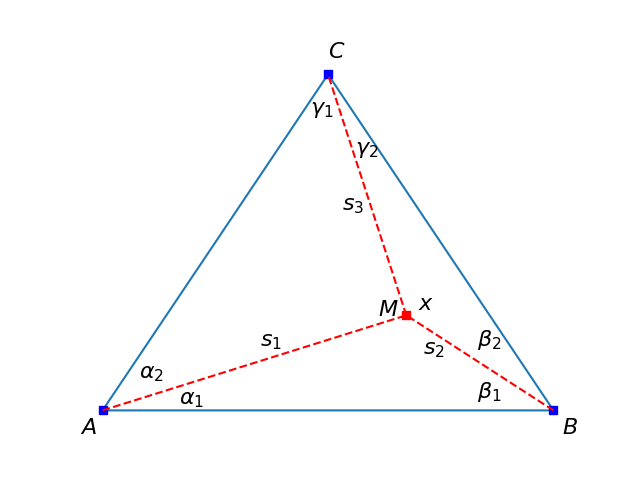
\includegraphics[width=1\textwidth]{figs/problem_statement.png}
\end{figure}

\begin{itemize}
\item $A$, $B$ and $C$ denote vertices
\item $s_1$, $s_2$ and $s_3$ denote the lengths of the line segments $AM$, $BM$ and $CM$, respectively
\item $\alpha_k$, $\beta_k$ and $\gamma_k$ for $k=1,2$ are angles
\item given are $\alpha_k$, $\beta_k$ ($k=1,2$)
\item $x$ (\emph{i.e.,} $\measuredangle BMC$) is the unknown
\end{itemize}

All angles are assumed to be in radians.

\section{Solution}

From triangle $ABM$ we have
\begin{align} \label{eq.abm_sin_theorem}
  \frac{s_1}{\sin \beta_1} = \frac{s_2}{\sin \alpha_1} \Rightarrow \frac{s_2}{s_1} = \frac{\sin\alpha_1}{\sin\beta_1}.
\end{align}
%
From triangle $AMC$ we have
\begin{align} \label{eq.amc_sin_theorem}
  \frac{s_3}{\sin \alpha_2} = \frac{s_1}{\sin \gamma_1} \Rightarrow s_3 = s_1\frac{\sin\alpha_2}{\sin\gamma_1}.
\end{align}
%
From triangle $BMC$ we have
\begin{align} \label{eq.bmc_sin_theorem}
  \frac{s_3}{\sin \beta_2} = \frac{s_2}{\sin \gamma_2} \Rightarrow s_3 = s_2\frac{\sin\beta_2}{\sin\gamma_2}.
\end{align}
%
Combining~\eqref{eq.amc_sin_theorem} and~\eqref{eq.bmc_sin_theorem} leads to
\begin{align} \label{eq.gamma_sin_ratio}
  \frac{\sin\gamma_2}{\sin \gamma_1} = \frac{s_2}{s_1} \frac{\sin\beta_2}{\sin\alpha_2}.
\end{align}
%
Let
%
\begin{align*}
  z = \frac{s_2}{s_1} \frac{\sin\beta_2}{\sin\alpha_2} = \frac{\sin\alpha_1}{\sin\beta_1} \frac{\sin\beta_2}{\sin\alpha_2},
\end{align*}
where we have used $s_2/s_1$ from~\eqref{eq.abm_sin_theorem}. Then~\eqref{eq.gamma_sin_ratio} can be expressed as
\begin{align}
  \sin\gamma_2 = z \sin \gamma_1,
\end{align}
%
and since $\gamma_1 + \gamma_2 = v \coloneqq \pi - (\alpha_1 + \alpha_2 + \beta_1 + \beta_2)$, we have
\begin{align}
  \sin\gamma_2 &= z \sin \gamma_1 \\
  &= z\sin(v - \gamma_2)\\
  &= \underbrace{z\sin v}_{c_1} \cos\gamma_2 - \underbrace{z\cos v}_{c2} \sin\gamma_2.
\end{align}
%
Hence
%
\begin{align}
  \frac{\sin \gamma_2}{\cos \gamma_2} = \tan \gamma_2 = \frac{c_1}{1 + c_2},
\end{align}
%
and we obtain
%
\begin{align}
  \gamma_2 = \arctan\left(\frac{c_1}{1 + c_2}\right).
\end{align}
%
Finally, $x = \pi - (\beta_2 + \gamma_2)$.

\nocite{*}
\bibliographystyle{ieeetr}
\bibliography{bib}

\end{document}
